\section{基于Elgamal签名方案的代理签名的实现}

\subsection{程序的模块划分}

\begin{figure}[H]
\centering
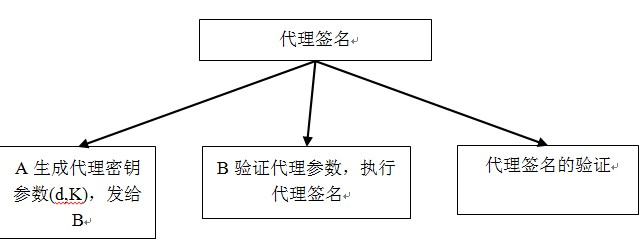
\includegraphics{img/4.jpg}
\caption{代理签名程序模块}
\end{figure}

\subsection{具体模块的实现}

\subsubsection{A授签名权给B的过程}

\begin{figure}[H]
\centering
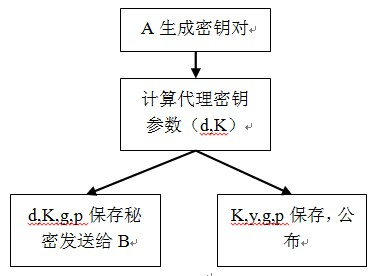
\includegraphics{img/5.jpg}
\caption{授权过程}
\end{figure}

A使用自定义函数void generateKey();生成大素数$p$,$g$,公钥$y$和私钥$x$;然后选择随机数$k$,计算$K = g^k$ $mod$ $p$:powmod(g, k, p, K);再计算$d = x + k*K$ $mod$ $p-1$:mad(k, K, x, p, p, d);(d,K)并将$d$,$K$,$g$,$p$存入proxy\_pri.txt,将$y$,$K$,$g$,$p$存入proxy\_pub.txt,以供后面程序调用数据。

\subsubsection{代理签名过程}

1)   B从proxy\_pri.txt中读取(d,K),并验证$g\textasciicircum d=y*K\textasciicircum k$ $mod$ $p$:
powmod(g, d, p, left); // $left = g\textasciicircum d$ $mod$ $p$  
powmod(K, K, p, temp); // $temp = K\textasciicircum K$ $mod$ $p$
mad(y, temp, temp,p,p, right);// $right = y*temp$ $mod$ $p = y*(K\textasciicircum K)$ $mod$ $p$
if (compare(left, right) != 0) return 0; else return 1;
     相等则接受代理。

2)  B使用代理私钥d对data.txt进行签名,先得到h= =messageHash1ToBig();

对h进行签名操作:
3)  取随机数$r$,要求$r$与$p-1$互素:
    irand((unsigned int)time(NULL));
    while (egcd(p-1, r ,b\_tmp)!=1) {bigrand(p-1, r);}
4)  计算R:调用MIRACL库函数powmod(g,r,p,R)计算$R=g\textasciicircum k$ $mod$ $p$;

5)  计算s:使用函数decr(p, 1, p);使接下来的p都变为p-1进行运算\cite{基于离散对数问题的代理数字签名};计算r逆元:xgcd(r,p,r,r,r);计算d=d*R,   h=h-d:multiply(R,x,x) , subtract(h,d,h); 计算$s=[r^-1*(h-Rd)]$ $mod$ $p-1$:mad(r, h, h, p, p, s);\cite{基于ELGamal体制的代理签名}

6)  丢弃r:mirkill(r);

7)  将所得的代理数字签名(R,s)存入proxy\_signature.txt

\begin{figure}[H]
\centering
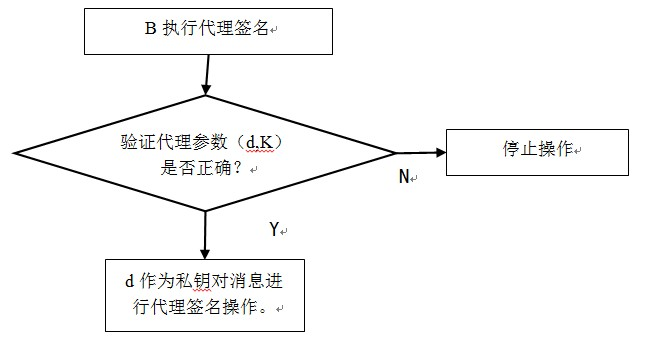
\includegraphics{img/6.jpg}
\caption{代理签名过程}
\end{figure}

\subsubsection{验证代理签名}

读取proxy\_signature.txt中的签名R和s;

2)    计算data.txt的h,h=messagehash1tobig();

3)    计算$g\textasciicircum h(mod$ $p)$并将值存入b\_tmp\_1:powmod(g,h,p,b\_tem\_1);
  
4)    计算$K=K\textasciicircum K$ $mod$ $p$:powmod(K, K, p, K);

5)    计算$temp = y*K$ $mod$ $p$:mad(y, K, K, p, p, temp);

6)    计算$(yK\textasciicircum K)\textasciicircum R*R\textasciicircum s$ $mod$ $p$并将值存入b\_tmp\_2:powmod2(temp, R, R, s, p, b\_tmp\_2);

7)    比较b\_tmp\_1和b\_tmp\_2的值,若相等则代理签名正确,接受签名,反之拒绝。
